%!TEX root = TFG.tex

\chapter{Estado del arte} \label{chap:art}

En este capítulo se introducirán los conceptos de dispositivos y arquitectura \acrshort{iot}, así como de Machine Learning. También se explicarán los algoritmos de aprendizaje utilizados en el desarrollo de este trabajo.

\section{Dispositivos IoT}

\subsection{Introducción}

El Internet de las Cosas, más conocido por Internet of Things (IoT), es el conjunto de  dispositivos capaces de conectarse a internet, recolectar e intercambiar datos de forma autónoma. Una cosa que distingue a los dispositivos IoT de los que no lo son, es que estos dispositivos pueden interactuar entre ellos sin necesidad de intervención humana.

El concepto de IoT fue primeramente mencionado por Kevin Ashton en 1999 mientras realizaba una presentación sobre dispositivos RFID \cite{gokhale2018introduction}. A pesar de esto el primer dispositivo de este tipo fue una máquina de refrescos en 1982 \cite{cokemachine1982iot}, que se conectaba a internet para informar los refrescos que contenía, y si estos se encontraban fríos.

\subsection{Arquitectura IoT}

Cada vez hay más dispositivos IoT conectados a internet, lo que dada su naturaleza, implica que son varias miles de millones de ellos. Por este motivo, los protocolos de la pila TCP/IP no están preparados para este número tan grande de dispositivos que manejar.

Existen diversas propuestas sobre arquitecturas multi capa que puedan asegurar los requisitos de calidad de servicio (QoS) y seguridad requeridos. En la propuesta de Muhammad Umar Farooq et al. \cite{farooq2015review} se hace mención a una arquitectura de 6 capas.

Por otro lado, en la propuesta de Ibrar Yaqoob et al. \cite{yaqoob2017internet} se explica una propuesta más general, combinando varias de las capas que comparten gran parte de su cometido. A continuación se explican estas 3 capas:

\begin{enumerate}
    \item \textbf{Capa sensitiva}: esta es la capa más básica. Es la que se encarga de recolectar toda la información que sea capaz el dispositivo a través de sus múltiples sensores.
    \item \textbf{Capa de transporte}: esta capa es la que realiza todo el intercambio de información entre las otras dos capas. Se encarga de las operaciones de red.
    \item \textbf{Capa de aplicación}: esta capa se encarga de extraer la información valiosa de los datos producidos por la capa sensitiva, y que le llegan a través de la capa de transporte. En esta capa se agrupan distintos servicios como data mining o computación en la nube.
\end{enumerate}

\subsection{Aplicaciones del IoT}

En la actualidad, se vive rodeados de dispositivos inteligentes. Estos dispositivos  permiten realizar todo tipo de acciones, por ejemplo, un teléfono móvil permite enviar y recibir emails, enviar mensajes instantáneos, utilizar redes sociales, etc. A pesar de todas esas funciones, todos estos aparatos comparten un ``problema'', necesitan de la intervención humana para realizar sus tareas.

De estas necesidades nacen los dispositivos IoT, por ejemplo, un frigorífico inteligente. Este frigorífico es capaz de llevar el inventario de productos que contiene y detectar cuando alguno de ellos está próximo a terminarse. De forma autónoma este dispositivo es capaz de conectarse a internet y realizar una pedido online al supermercado de nuestra preferencia para reabastecerse de estos productos.

Este es sólo un ejemplo, dentro del hogar se pueden encontrar también los muy conocidos robots aspiradora o los asistentes inteligentes, pero estos dispositivos pueden ir mucho más lejos. Estos dispositivos se pueden usar para un control inteligente del tráfico, donde un coche autónomo puede recibir en tiempo real las rutas menos congestionadas que seguir hacia un destino.

Otro de sus posibles usos está en la medicina. Donde se pueden instalar dispositivos de este tipo para medir distintas métricas de salud de los pacientes, como la frecuencia cardíaca o el nivel de glucosa en sangre. De esta forma, en caso de que una persona presente algún desorden, una ambulancia puede ser avisada de forma inmediata aunque dicha persona esté sola e inconsciente.

Como último ejemplo se mencionará al sector agrícola. En este campo se pueden desplegar drones que detecten el nivel de humedad del terreno y, por ejemplo, activen el riego de cierta zona en caso de ser necesario. También pueden haber sensores a nivel del suelo que detecten la calidad del suelo, midiendo los distintos nutrientes y actuando en consecuencia.

\section{Machine Learning}

\subsection{Introducción}

El Machine Learning se trata de una búsqueda, una búsqueda de formas alternativas de hacer algo. Para ello se busca en estructuras muy similares a las previas. Para modificar una estructura y seguir con la búsqueda nos valemos de sucesos que hayan acontecido, entonces, evaluamos si han mejorado y nos quedaremos como estructura para la siguiente iteración con la que más mejore a la previa. Para realizar estas operaciones necesitamos una forma de cambiar de estructura y una forma de evaluar si hemos mejorado.

Con esta forma de trabajar se puede ver que el programa no tiene que resolver la tarea sino autoajustarse para obtener mejores evaluaciones cada vez. El programador por tanto no pone el programa sino proporcionar al programa la mejor estructura modificable y a continuación alimentar al sistema con datos. Aportamos por tanto ejemplos o premios que ayudan al programa a autoajustarse. Existen tres tipos de aprendizaje: 

\begin{itemize}
    \item \textbf{Supervisado}: al sistema se le proporcionan ejemplos de cuales la solución es conocida. Una variante sería el semi-supervisado en el que sólo una parte de los datos tienen solución conocida.
    \item \textbf{No Supervisado}: al sistema se le proporcionan datos que no tienen una solución conocida, esperando que el sistema nos proporcione conocimiento que intuimos que existe en dichos datos. Un ejemplo sería el \textit{clustering} que agrupa los datos por similitudes.
    \item \textbf{Por refuerzo}: al sistema no se le pasan ejemplos de datos, sino que se le premia o castiga por distintas conductas que desarrolla automáticamente. Al final el sistema, que busca obtener más premios, se comportará de la forma que queremos.
\end{itemize}

\subsection{Tratamiento de los datos}

Para obtener un resultado de cuan bueno es un modelo (algoritmo) que se quiere usar se debe dividir el conjunto de datos inicial en dos conjuntos: \textbf{datos de entrenamiento} y \textbf{datos de test}. Con los datos de entrenamiento el algoritmo se ajusta y aprende de los ellos, y con los datos de test se analizan los resultados obtenidos del algoritmo ante datos que no ha visto antes.

Para realizar una comparación entre distintos modelos donde se quiere ver cual es el que mejor se ajusta a los datos se debe dividir el conjunto de datos de entrenamiento en otros dos conjuntos: \textbf{conjunto de entrenamiento} y \textbf{conjunto de validación}. Con este último se puede evaluar la capacidad de generalizar de nuestro algoritmo.

Con esta segunda división se obtiene el algoritmo que mejor se adapta a los datos, pero no un modelo final. Para tener un modelo final se entrenará este con el conjunto de datos de entrenamiento en su totalidad y se evaluará con los datos de test.

\subsection{Algoritmos de aprendizaje supervisado} \label{sec:algorithms}

Dentro de los algoritmos de aprendizaje supervisado se encuentran algoritmos que clasifican y algoritmos que se dedican a la regresión.

Los algoritmos clasificadores tratan de agrupar a los distintos vectores de entrada en distintas clases. Un ejemplo de esto sería un algoritmo de clasificación binaria, en la que existen ejemplos \textbf{positivos} (pertenecen a la clase) o \textbf{negativos} (no pertenecen). Esto genera los conceptos de \textbf{falso positivo} (el sistema dice que pertenece y es falso) y \textbf{falso negativo} (el sistema dice que no pertenece y es falso).

Los algoritmos regresores buscan dar una salida numérica como resultado en lugar de la pertenencia a una clase, por tanto no sirven para este trabajo. A continuación se explicarán los algoritmos que se han usado para el desarrollo de este trabajo.

\subsubsection{Árboles de decisión}

La idea principal del algoritmo es que partiendo de un conjunto de elementos en el nodo padre, haciendo una pregunta binaria tal que se pude dividir el conjunto en otros 2 que sean más puros, es decir, que los elementos entre sí compartan (al menos) la característica por la que hemos preguntado.

Si los atributos son categóricos se puede crear una partición diciendo si pertenecen o no a la clase. Por contra, si los atributos son ordinales se pueden tener preguntas del tipo $x \leq x_c$.

\subsubsection{Random Forest}

Este algoritmo es un conjunto de árboles de decisión trabajando en paralelo. Cada árbol realizará de forma aleatoria una partición distinta a los otros para cada división de una rama, con esto se obtiene variabilidad en los resultados de los árboles. Por último, el algoritmo toma como salida aquella clase que haya sido el resultado de más árboles.  \cite{hatwell2020chirps} \cite{breiman2001random}

\subsubsection{Multilayer Perceptron (MLP)}

Se trata de un modelo de red neuronal artificial de tipo \textit{feed-forward} (es decir, no existen ciclos en el grafo que forma la red). Consiste en una serie de múltiples capas (multilayer) de nodos que conforman grafos dirigidos, estando cada capa conectada con la siguiente. 

MLP entrena la red utilizando la propagación hacia atrás (backpropagation) que, empleada junto con una técnica de optimización como gradient descent, calcula el gradiente de una función de pérdida respecto a todos los pesos en la red, de manera que se pasa el valor del gradiente al método de optimización y este lo usa para actualizar los pesos, con el objetivo de minimizar la función de pérdida.

\subsubsection{Naive Bayes}

Los algoritmos de aprendizaje bayesianos tratan de encontrar la probabilidad de que un dato pertenezca a una clase. Una vez se tienen todas las probabilidades de pertenencia a una clase se toma como salida del algoritmo aquella clase con la mayor probabilidad.

Para realizar este proceso el algoritmo usa distintos atributos de cada dato $a_1, \dots, a_n$. Ahora este proceso se trata de conoces la probabilidad condicionada de que este conjunto de atributos pertenezca a una determinada clase. Esto es muy costoso y por tanto hay que relajar esta hipóstesis. Para ello se asume independencia entre los atributos de ahí el nombre de \textit{naive}.

\subsubsection{K Nearest Neighbours (KNN)}

El algoritmo KNN es un algoritmo que se usa mayoritariamente para clasificación. En este algoritmo los datos se agrupan por distancias.

A la hora de clasificar un nuevo dato, este algoritmo busca los $k$ datos más cercanos. Una vez tiene esos datos comprueba sus clases. La clase con mayor representación entre los $k$ datos es la que se asignará al nuevo dato. Podemos verlo con un ejemplo.

\begin{figure}[htpb!]
    \centering
    \begin{tikzpicture}
        \node (1) {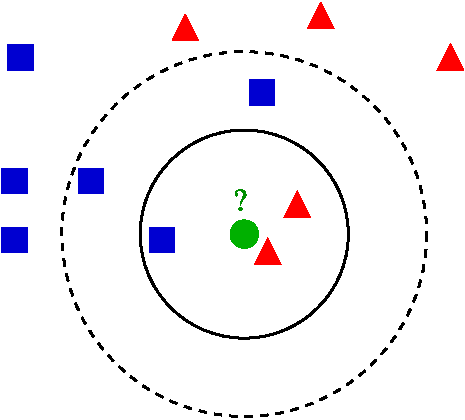
\includegraphics[width=0.4\textwidth]{images/KnnClassification}};
        \node (2) at (0.2, -1.3) {$k = 3$};
        \node (3) at (0.2, -2.6) {$k = 5$};
    \end{tikzpicture}
    \caption{Funcionamiento del algoritmo KNN \cite{knnalgorithm2010}}
    \label{fig:knn_clasification}
\end{figure}

En la Fig. \ref{fig:knn_clasification} se quiere clasificar el dato \textcolor{verdedato}{\Large$\bullet$}, una opción es usar múltiples valores de $k$ y con ello obtener diferentes resultados:
\begin{itemize}
    \item Asignando $k = 3$ sólo se tendrán en cuenta los 3 datos más próximos, que serán 2 de la clase \textcolor{rojodato}{\large$\blacktriangle$} y uno de la clase \textcolor{azuldato}{$\blacksquare$}. Con esto la clase que se asignará al dato \textcolor{verdedato}{\Large$\bullet$} será \textcolor{rojodato}{\large$\blacktriangle$}.
    \item Asignando $k = 5$ sólo se tendrán en cuenta los 5 datos más próximos, que serán 2 de la clase \textcolor{rojodato}{\large$\blacktriangle$} y tres de la clase \textcolor{azuldato}{$\blacksquare$}. Con esto la clase que se asignará al dato \textcolor{verdedato}{\Large$\bullet$} será \textcolor{azuldato}{$\blacksquare$}.
\end{itemize}

\subsubsection{Máquinas de vector soporte (SVM)}

Las máquinas de vector soporte son un conjunto de algoritmos de aprendizaje supervisado que se utilizan tanto para clasificación como para regresión, en este caso se analizará únicamente en clasificación.

Estos algoritmos toman los datos como puntos en un espacio $n-$dimensional. El objetivo es dividir estos datos mediante hiperplanos de forma que los puntos que contenidos en una región del espacio delimitada por los mismos hiperplanos sean una misma clase y que estén lo más separados posible. Esto se puede ver más fácil con un ejemplo.

En la Fig. \ref{fig:svm_separation} se puede ver como hay distintos hiperplanos ($\mathcal{H}_1, \mathcal{H}_2, \mathcal{H}_3$) que pueden dividir el espacio. 

\begin{itemize}
    \item $\mathcal{H}_1$ no divide de forma correcta todos los puntos de la entrada, puesto que hay puntos negros juntos con blancos.
    \item $\mathcal{H}_2$ sí que divide a todos los puntos en dos clases de la forma correcta, pero no están seraparas lo máximo posible de este hiperplano.
    \item $\mathcal{H}_3$ sí que cumple con las restricciones de división y distancia máxima.
\end{itemize}

\begin{figure}[htpb!]
    \centering
    \begin{tikzpicture}
        \node (1) {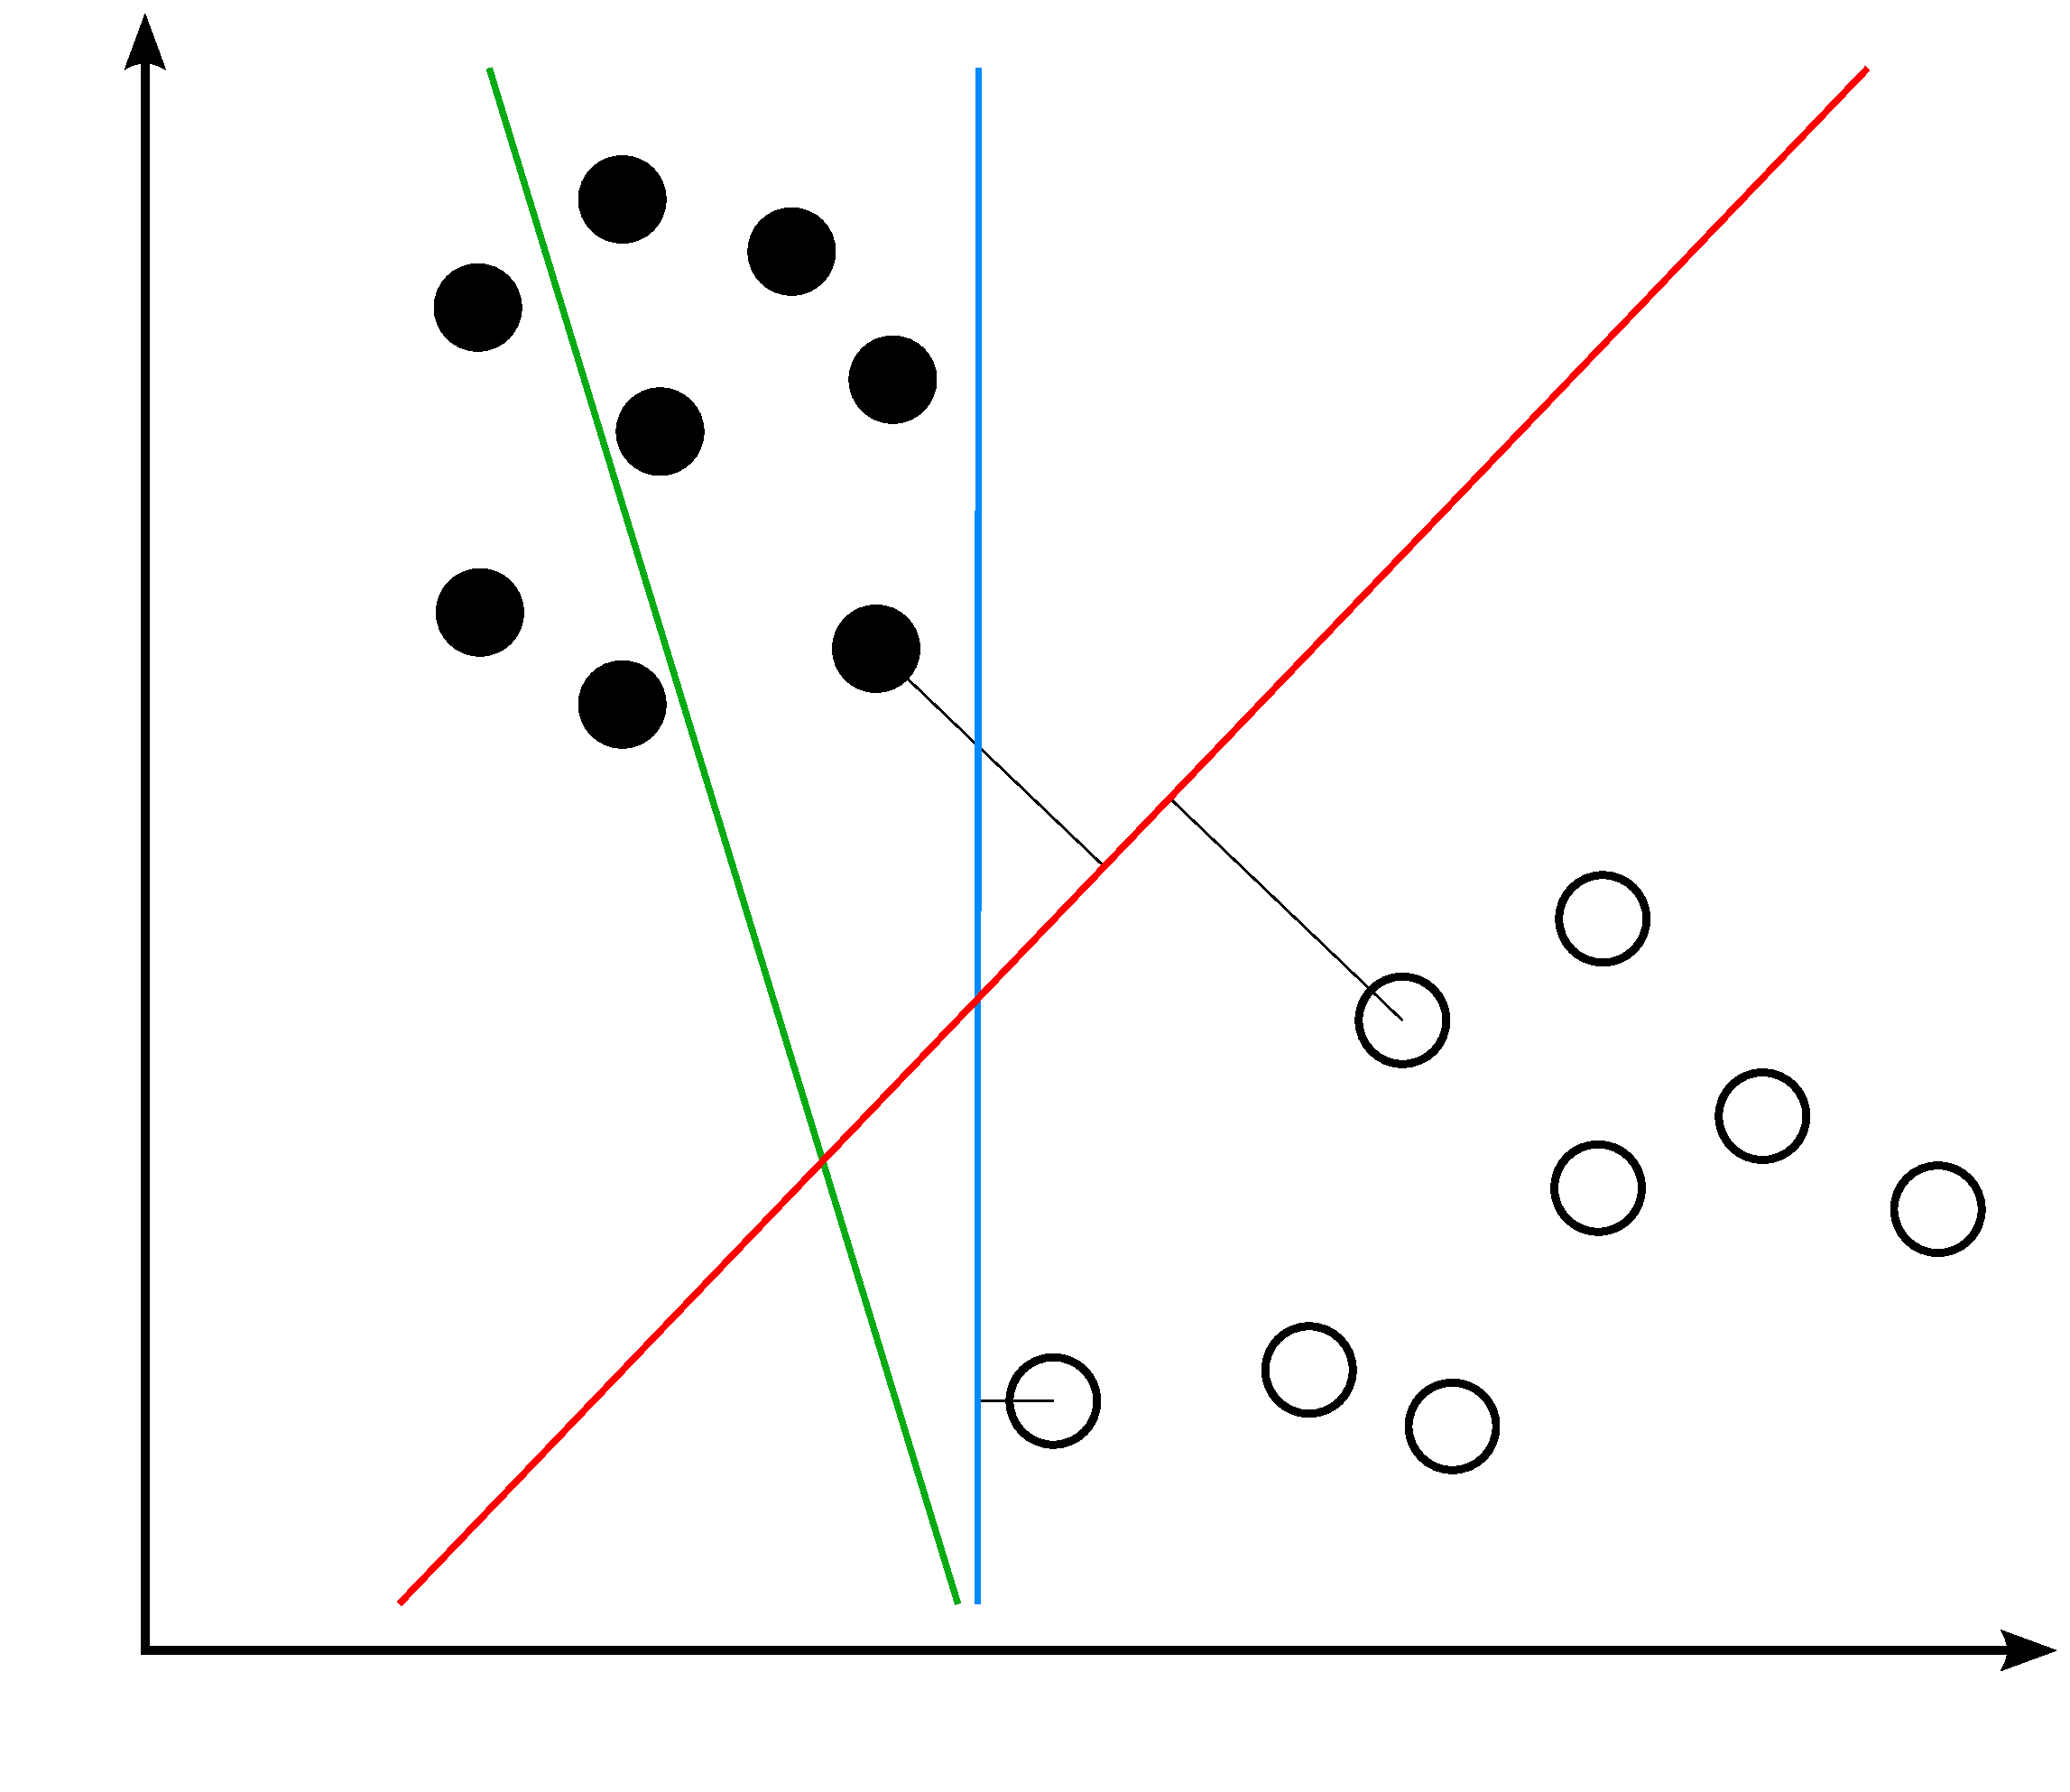
\includegraphics[width=0.4\textwidth]{images/svm_separation}};
        \node (2) at (2.7, -2.7) {$x_1$};
        \node (3) at (-3.2, 2.2) {$x_2$};
        \node (4) at (-2, 2.5) {\scriptsize $\mathcal{H}_1$};
        \node (5) at (-0.5, 2.5) {\scriptsize $\mathcal{H}_2$};
        \node (6) at (2, 2.5) {\scriptsize $\mathcal{H}_3$};
    \end{tikzpicture}
    \caption{Separación por hiperplanos SVM \cite{svmseparation2012}}
    \label{fig:svm_separation}
\end{figure}

En muchas ocasiones no se podrán dividir los conjuntos de forma correcta usando únicamente divisiones lineales del espacio, por ello, habrá que usar divisiones no lineales.

\section{Revisión bibliográfica}

En esta sección se realiza un estudio del estado del arte relativo a la aplicación de distintas técnicas que tengan como objetivo identificar a un dispositivo a través de la red independientemente de un identificador susceptible de ser identificado. Para estos cometidos son muy utilizados los algoritmos de aprendizaje automático o Machine Learning. 

Para comenzar la revisión bibliográfica, se analizará el trabajo desarrollado por Pascal Oser et al. \cite{oser2018identifying}. En este trabajo se desarrolla un sistema para identificar dispositivos entre un total de 562 en el centro del CERN. Para este cometido se tomas muestras periódicas de las marcas de tiempo (timestamps) contenidas en paquetes TCP que se envían y reciben de estos dispositivos.

De estas marcas se obtienen las variables que se usarán para entrenar los distintos modelos de machine learning. Las variables que obtiene son el incremento entre dos marcas consecutivas, el desbordamiento del contador de la marca de tiempo, la mediana de todas las marcas, etc.

Una variable interesante es la del desbordamiento del contador. En el RFC 1323 \cite{RFC1323} se define que el contador del timestamp (campo TSval) tiene una longitud de 4 bytes (32 bits), por lo tanto, el mayor valor que podrá tener asignado es $2^{32}$, puesto que es un entero sin signo. Se podría pensar que todos los dispositivos desbordan a la vez, pero cada fabricante establece el valor al que el contador se desborda. Esto está ilustrado en la Fig. \ref{fig:cern_ts_overflow} con dos ejemplos.

\begin{figure}[htpb!]
    \centering
    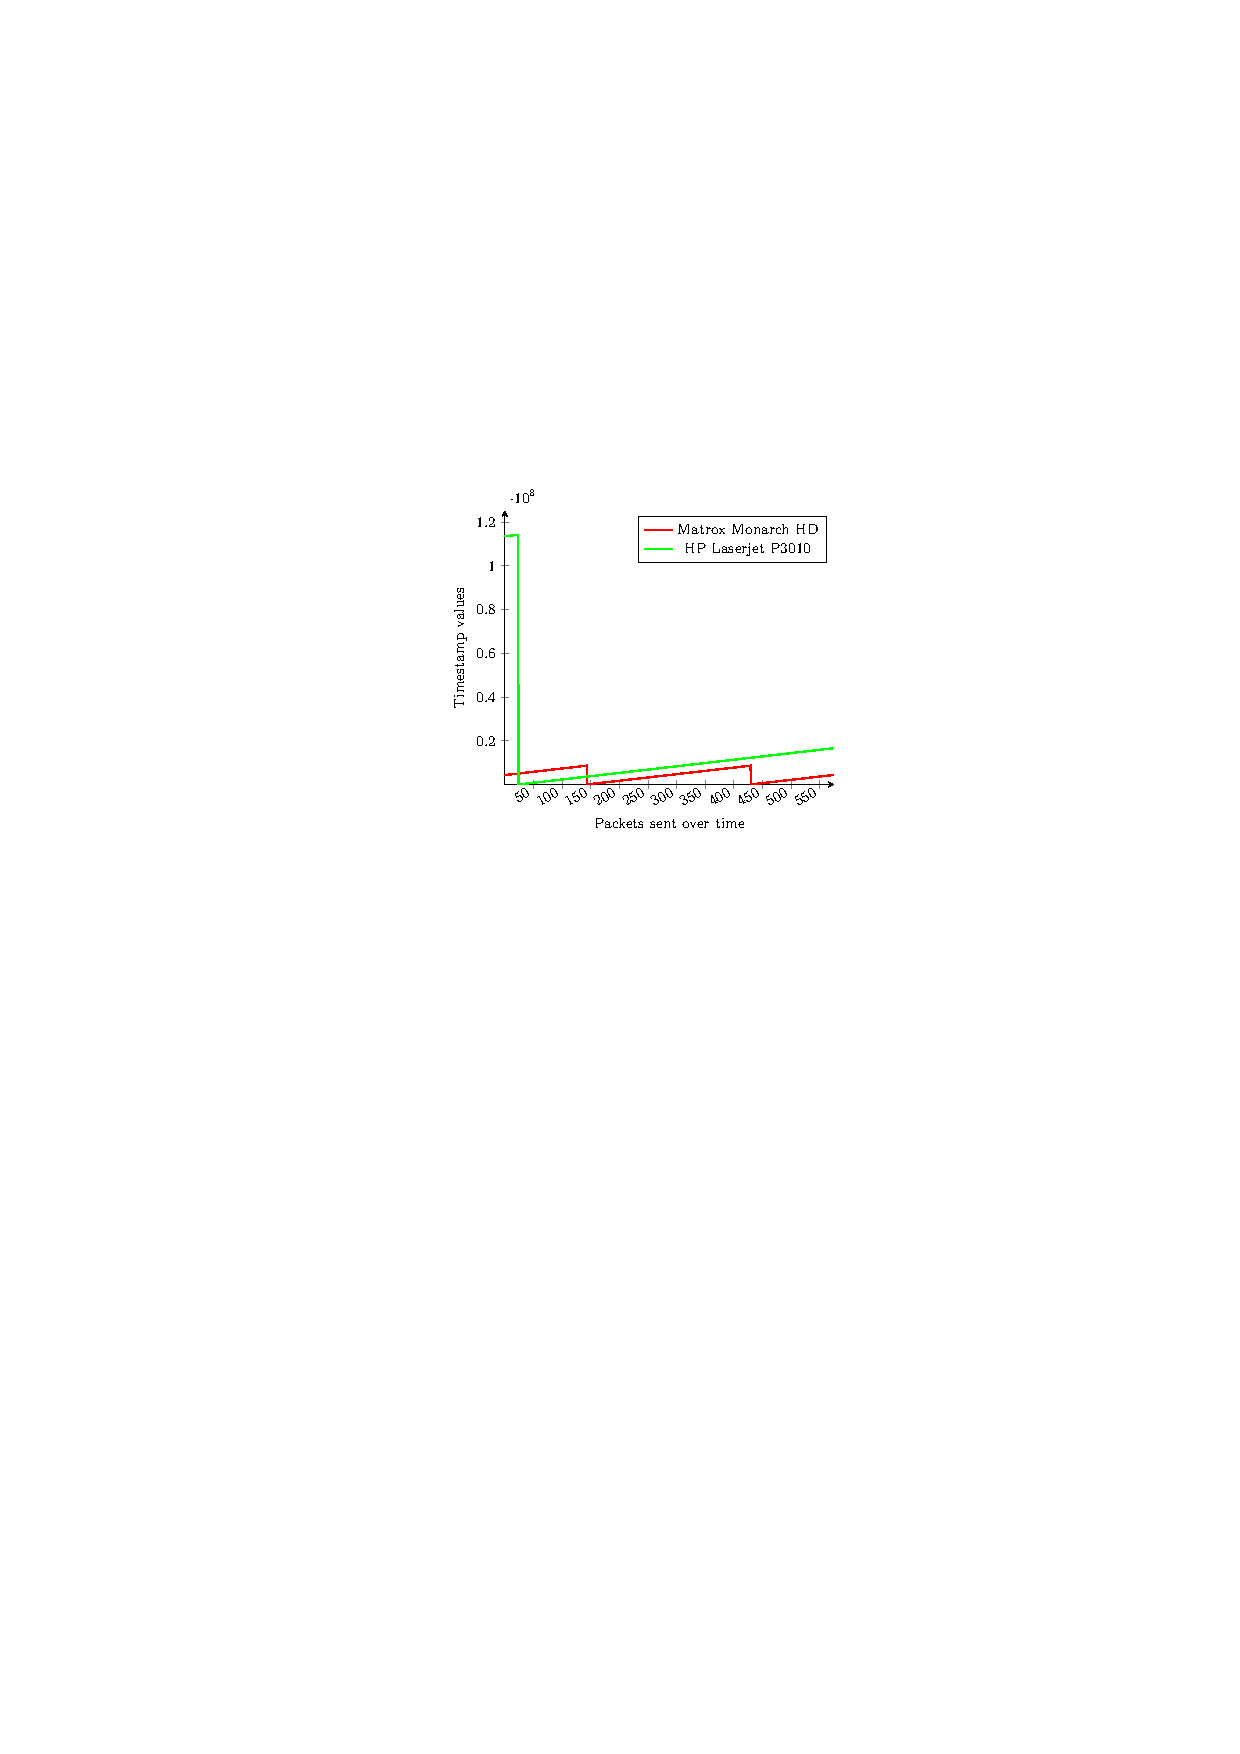
\includegraphics[width=0.45\textwidth]{images/CERN-timestamp_overflow}
    \caption{Desbordamiento del contador \cite{oser2018identifying}}
    \label{fig:cern_ts_overflow}
\end{figure}

Una vez tiene todas las variables registradas para todos los dispositivos, compara varios modelos de machine learning, para clasificar cada uno de los dispositivos. Los resultados que obtiene son de un accuracy del 99.22\% con MLP, un 99.14\% con SVM y por último 99.67\% con Random Forest.

Con estos datos decide quedarse con el modelo de Random Forest, el cual entrena con la totalidad de los datos de entrenamiento, obteniendo finalmente una precisión del 97.03\% y un accuracy del 99.76\%.

Otro trabajo relacionado con la temática ha sido desarrollado por Salma Abdalla Hamad et al. \cite{hamad2019iot}. En este trabajo se desarrolla un sistema que identifique a un dispositivo que quiere conectarse a la red y decida si se le permite realizar esta acción o se le deniega. Además este sistema comprobará periódicamente los dispositivos que están ya en la red para detectar comportamientos malintencionados. 

Este sistema (Fig. \ref{fig:diam_hamad}), una vez se tiene una traza del dispositivo que se quiere conectar por primera vez a la red, crea una huella del dispositivo que será analizada por un modelo (previamente entrenado) que lo clasificará como desconocido o no, en caso de que esté en una lista blanca. En caso de ser un dispositivo desconocido se le denegará el acceso a la red. Por contra, si está en la lista, se consultará una matriz de autorización (que contiene la confianza de ese dispositivo según sus vulnerabilidades) para saber que privilegios recibirá ese dispositivo. Con esto el dispositivo puede contectarse como un dispositivo ``confiable'', teniendo acceso a comunicarse con todos los dispositivos de la red, o por contra, de ``acceso restringido'' donde solo podrá comunicarse con dispositivos de ese mismo nivel de acceso.

\begin{figure}[htpb!]
    \centering
    \resizebox{0.6\textwidth}{!}{
        \begin{tikzpicture}
    \node[draw, text width = 2cm, align = center, minimum width = 2cm, fill = blancodiagrama, execute at begin node=\setlength{\baselineskip}{1em}] (1) {\footnotesize Sequence Capture};
    \node (2) [left = 3cm of 1] {};
    \node[draw, rounded corners, fill = azuldiagrama] (3) [below = of 1] {\footnotesize Finger Print};
    \node[draw, diamond, aspect = 2, fill = azuldiagrama] (4) [below = of 3] {\footnotesize Classifier};
    \node[draw, cylinder, rotate = 90, fill = verdediagrama, minimum height = 0.5cm, minimum width = 0.5cm, scale = 0.5] (5) at (-0.9,-3.85) {};
    \node[draw, rounded corners, fill = azuldiagrama] (6) [below = of 4] {\footnotesize Zoning};
    \node (7) [left = 3cm of 6] {};
    \node (8) [below = of 6] {};
    \node[draw, fill = verdediagrama] (9) [left = of 8] {\footnotesize Trusted};
    \node[draw, fill = naranjadiagrama] (10) [right = of 8] {\footnotesize Restricted};
    \node[draw, text width = 2cm, align = center, minimum width = 2cm, fill = blancodiagrama, execute at begin node=\setlength{\baselineskip}{1em}] (11) [below = of 8] {\footnotesize Random Capture};
    \node[draw, rounded corners, fill = azuldiagrama] (12) [below = of 11] {\footnotesize Finger Print};
    \node[draw, diamond, aspect = 2, fill = azuldiagrama] (13) [below = of 12] {\footnotesize Classifier};
    \node[draw, cylinder, rotate = 90, fill = verdediagrama, minimum height = 0.5cm, minimum width = 0.5cm, scale = 0.5] (14) at (-0.9,-12.73) {};
    \node[draw, ellipse, minimum height = 1.5cm, fill = verdediagrama] (15) [left = of 13] {\footnotesize Match};
    \node[draw, fill = rojodiagrama] (16) [left = 2.5cm of 9] {\footnotesize Rejected};
    \node[draw, fill = rojodiagrama] (17) [right = 2.5cm of 10] {\footnotesize Quarantine};
    \node (18) [above right = 4.7cm of 13] {};
    \node (19) [below right = 0.7cm of 13] {};
    
    \draw (2) -- (1) node [midway, above, text width = 2.5cm, align = center] {\footnotesize Unseen Device Network Traces};
    \draw (2) -- (1) node [midway, below, text width = 2.5cm, align = center] {\footnotesize 010111000011001};
    \draw (1) -- (3);
    \draw (3) -- (4);
    \draw (4.west) -| (16.north) node [pos=0.25, above] {\footnotesize Unknown Device};
    \draw (4) -- (6);
    \draw (7) -- (6) node [above, midway] {\scriptsize Authorisation Matrix};
    \draw (6) -- (9);
    \draw (6) -- (10);
    \draw (9) -- (11);
    \draw (10) -- (11);
    \draw (11) -- (12);
    \draw (12) -- (13);
    \draw (15) -- (13);
    \draw (13) -| (18.center) node [pos=0.25, above] {\footnotesize Mis-Classified} |- (6);
    \draw (13) |- (19.center) -| (17) node [pos=0.17, above] {\footnotesize Suspicious/Mis-Behaving};
\end{tikzpicture}
    }
    \caption{Modelo del sistema de identificación \cite{hamad2019iot}}
    \label{fig:diam_hamad}
\end{figure}

Para los dispositivos que ya están conectados a la red, se toma una muestra aleatoria que comprobará si se han clasificado de forma correcta. En el caso de que se haya clasificado mal pero siga estando en la lista blanca se actualizará su matriz de autorización. Por otra parte, en caso de que no esté en dicha lista se pondrá en cuarentena para ser analizado más adelante.

Las huellas de los dispositivos se obtienen del payload de los mensajes enviados por ese dispositivo. De ellos se obtienen 67 características como el tamaño del paquete Ethernet, el tamaño de las cabeceras, la IP de destino, el TTL, etc.

Con estas huellas entrena distintos modelos como son AdaBoost, LDA, KNN, Árboles de decisión, Naive Bayes, SVM, Random Forest y GBoost. Obtuvo un accuracy final del 89\%.

El siguiente artículo que se analizará es el realizado por Ahmet Aksoy et al. \cite{aksoy2019automated}. Este trabajo diseña un sistema (llamado SysID) que es capaz de identificar dispositivos a través del tráfico de red. 

Este sistema únicamente necesita un paquete de red para identificar el dispositivo. Dado un paquete de la traza se seleccionan $n$ cabeceras del paquete mediante un algoritmo genético, que implementa una función fitness (Eq. \ref{eq:aksoy_fit}) que trata de reducir este número de cabeceras. 

\begin{equation}
    Fitness = 0.9 \cdot Accuracy + 0.1 \cdot \left( 1 - \frac{\lvert SelectedFeatures \rvert - 1}{\lvert AllFeatures \rvert - 1} \right)
    \label{eq:aksoy_fit}
\end{equation}
donde $n = \lvert SelectedFeatures \rvert$ y $Accuracy$ es el resultado que se obtiene del modelo de machine learning entrenado con esas cabeceras.

Las trazas que se han usado para clasificar estos dispositivos provienen de una base de datos de otro artículo \cite{miettinen2017iot}, de donde se obtienen 20 medidas de 23 dispositivos IoT.

Para la clasificación se han usado diferentes algoritmos de la herramienta WEKA \cite{hall2009weka} como son tablas de decisión, árboles de decisión J48, OneR y PART. Se decide usar una clasificación en dos niveles (Fig. \ref{fig:askoy_classifier}), se clasifican primero entre su proveedor o el propio dispositivo, dependiendo de si hay más de un mismo dispositivo del mismo proveedor. Después se clasifican los dispositivos del mismo proveedor entre sí. Este esquema ayuda a tener mejores resultados pues cada proveedor puede ser identificado de mejor forma por un algoritmo distinto.

Los resultados que obtiene son de un 82\% de accuracy promedio entre todos los clasificadores de cada proveedor. Los valores individuales están entre el 42.2\% y el 100\%.

\begin{figure}[htpb!]
    \centering
    \resizebox{0.6\textwidth}{!}{
        \begin{tikzpicture}
    \node[draw, fill = azulclasificador, minimum width = 4.5cm] (0) {Hue Classifier};
    \node[draw, fill = azulclasificador, minimum width = 4.5cm] (1) [left = of 0] {Device Genre Classifier};
    \node[draw, fill = azulclasificador, minimum width = 4.5cm] (2) [above = 0.4cm of 0] {EdimaxPlug Classifier};
    \node[draw, fill = azulclasificador, minimum width = 4.5cm] (3) [above = 0.4cm of 2] {D-Link Classifier};
    \node[draw, fill = azulclasificador, minimum width = 4.5cm] (4) [below = 0.4cm of 0] {TP-Link Classifier};
    \node[draw, fill = azulclasificador, minimum width = 4.5cm] (5) [below = 0.4cm of 4] {Smarter Classifier};
    \node[draw, diamond, shape aspect = 2, fill = rojoclasificador] (6) [below = 0.4cm of 5] {Result};
    \node[draw, diamond, shape aspect = 2, fill = rojoclasificador] (7) [right = of 0] {Result};
    \node[draw, tape, tape bend top = none, tape bend height = 6pt, text width = 2.3cm, align = center, fill = verdeclasificador] (8) [above = 1.72cm of 1.west, anchor = west] {Arff file \\ (All devices)};
    
    \draw (1) -- (0);
    \draw (1.north) to [bend left = 18] (2.west);
    \draw (1.north) to [bend left] (3.west);
    \draw (1.south) to [bend right = 18] (4.west);
    \draw (1.south) to [bend right] (5.west);
    \draw (1.south) to [bend right] (6.west);
    
    \draw (0) -- (7);
    \draw (3.east) to [bend left] (7.north); 
    \draw (2.east) to [bend left] (7.north west); 
    \draw (4.east) to [bend right] (7.south west); 
    \draw (5.east) to [bend right] (7.south); 
    
    \draw (8) -- (8 |- 1.north);
\end{tikzpicture}
    }
    \caption{Clasificador de dos niveles \cite{aksoy2019automated}}
    \label{fig:askoy_classifier}
\end{figure}

El siguiente trabajo que se verá es el realizado por Hossein Jafari et al. \cite{jafari2018iot}. En este artículo no se utilizan paquetes de la capa de red o transporte, sino de la capa física. Para realizar esta labor se obtendrá la huella de cada dispositivo mediante radio frecuencias, por esta razón, este estudio sólo se centrará en conexiones inalámbricas, en este caso 6 dispositivos ZigBee \cite{gislason2008zigbee}.

Para cada uno de los dispositivos se realiza una captura de 5 minutos. Esta captura será del SNR en 5 niveles distintos, con lo que se obtiene \SI{10}{\giga\byte} por dispositivo y nivel de SNR, lo que en total serían \SI{300}{\giga\byte} de datos.

A continuación procede a entrenar tres modelos de deep learning, DNN, CNN y LSTM (los tres modelos pertenecen a la librería \texttt{TensorFlow} programada para Python \cite{tensorflow2015-whitepaper}), con los que obtiene unos resultados de 96.3\%, 94.7\% y 76\% respectivamente.

Fabian Lanze et al. \cite{lanze2012clock} han desarrollado un trabajo en el que crean un sistema de identificación de dispositivos basado en el clock skew. Su objetivo es generar huellas para cada punto de acceso, de forma que si un dispositivo pueda saber si ese punto de acceso es legítimo, o por contra si puede ser un potencial atacante.

Lo primero que hacen es definir el skew de un reloj como la primera derivada del offset de dicho reloj. De forma práctica usarán la desviación que almacena el demonio del servicio NTP para aproximar el skew del dispositivo conectado al punto de acceso. Usará conexión inalámbrica y recogerá hasta 6000 paquetes por dispositivo en cada muestra (10 minutos). Si en una muestra no se alcanzan los 500 paquetes, por problemas de conexión o cualquier otro motivo, esa muestra se elimina. Con este proceso se consiguen medir 388 puntos de acceso. 

Finalmente, trata de generar una huella para cada punto de acceso de forma estadística, basándose sobre todo en la distribución del clock skew. Como resultado obtiene que su método no es suficientemente preciso y que muchos dispositivos presentan una huella similar, por lo tanto, concluye que no es posible identificarlos únicamente de esta forma.

En el trabajo desarrollado por Yair Meidan et al. \cite{meidan2017profiliot} se desarrolla un sistema que es capaz de identificar dispositivos IoT a través de su tráfico de red. Las pruebas se realizan con trazas sobre conexión inalámbrica y tanto con dispositivos IoT como con PCs, smartphones, etc. 

De estas trazas se centran específicamente en las sesiones TCP, donde cada una se representa como un conjunto de características de cada paquete.

Primeramente, ejecutan un clasificador binario con el que obtienen la probabilidad de que un dispositivo sea IoT, usando solo información de una sesión TCP de cada dispositivo. En este apartado obtienen un \SI{100}{\percent} de acierto.

Por último, entrenan distintos modelos de clasificación (GBM, Random Forest, XGBoost), únicamente sobre los dispositivos previamente etiquetados como IoT, obteniendo finalmente un resultado de un \SI{99.281}{\percent} de accuracy en la identificación del modelo y marca de cada uno de ellos.

Como último artículo se analizará la propuesta realizada por Loh Chin Choong Desmond et al. \cite{desmond2008identifying}. En este trabajo han construido un sistema de identificación de dispositivos basado en los mensajes \textit{probe request} de los distintos dispositivos. Para ello, distinguirán como dispositivos distintos las distintas combinaciones de la tupla: $\langle$``Machine'', ``Wireless Network Interface Card (NIC) Driver'', ``Operating System''$\rangle$.

A continuación, comprueban que en el tiempo de emisión de estos mensajes se ven varios comportamientos que se repiten. Luego, observan que la latencia entre ráfagas de estos mensajes también presenta estos comportamientos distintivos. Con estas latencias son con las que entrenarán un modelo que sea capaz de distinguir los dispositivos.

El modelo que eligen se basa en aprendizaje no supervisado, Maximum Variance Clustering \cite{veenman2002maximum}. Este modelo es similar al algoritmo de $k$-medias, la distinción es que $k$-medias necesita conocer previamente el número de clústeres $k$ previamente, mientras que Maximum Variance Clustering necesita conocer la varianza máxima dentro de un clúster $\sigma^2_{max}$. Con este algoritmo obtienen unos resultados de accuracy entre el \SI{70}{\percent} y el \SI{80}{\percent}.


\subsection{Resultados de la revisión bibliográfica}

Por último se realizará un resumen en forma de tabla de los artículos que han sido revisados. 

\begin{table}[t]
    \centering
    \resizebox{\textwidth}{!}{
        \begin{tabular}{C{0.12\textwidth}C{0.15\textwidth}C{0.15\textwidth}C{0.15\textwidth}C{0.14\textwidth}C{0.2\textwidth}C{0.24\textwidth}}
            \toprule
            Referencia & Tipo de identificación & Fuente de los datos & Método de clasificación & Tipo de aprendizaje & Algoritmos usados & Resultados \\
            \midrule
            \cite{oser2018identifying} & Tipo de dispositivo & Cabeceras TCP & Machine Learning & Supervisado & MLP, SVM, Random Forest & 99.76\% de accuracy y 97.03\% de precisión \\
            \addlinespace\addlinespace
            \cite{hamad2019iot} & Individual & Característi-cas del payload & Machine Learning & Supervisado & AdaBoost, LDA, KNN, Árboles de decisión, Naive Bayes, SVM, Random Forest y GBoost & 89\% de accuracy \\
            \addlinespace\addlinespace
            \cite{aksoy2019automated} & Tipo y modelo del dispositivo & Cabereceras TCP & Machine Learning & Supervisado & Tablas de decisión, Árboles de decisión J48, OneR y PART & Entre 42.2\% y 100\% de accuracy, con un promedio de 82\% \\
            \addlinespace\addlinespace
            \cite{jafari2018iot} & Individual & Radio frecuencias & Machine Learning & Supervisado & DNN, CNN y LSTM & 96.3\% de accuracy en DNN, 94.7\% de accuracy en CNN y 76\% de accuracy en LSTM \\
            \addlinespace\addlinespace
            \cite{lanze2012clock} & Modelo del dispositivo & Registros NTP & Estadístico & - & - & Inconcluyentes \\
            \addlinespace\addlinespace
            \cite{meidan2017profiliot} & Tipo y modelo & Sesiones TCP & Machine Learning & Supervisado & GBM, Random Forest y XGBoost & \SI{99.281}{\percent} de accuracy \\
            \addlinespace\addlinespace
            \cite{desmond2008identifying} & Individual & Mensajes \textit{probe request} & Machine Learning & No supervisado & Maximum Variance Clustering & Entre un 70\% y 80\% de accuracy\\
            \addlinespace\addlinespace
            Este trabajo & Individual & Ciclos de CPU & Machine Learning & Supervisado y No supervisado & Random Forest, MLP, Naive Bayes, KNN, Árboles de decisón, SVM-Linear, LOF, OC-SVM, Isolation Forest & 99.38\% de Accuracy, 99.39\% de Recall y 99.38\% de $f$-score\\
            \bottomrule
        \end{tabular}
    }
    \caption{Resultados en el estado del arte}
    \label{tab:art_results}
\end{table}


